\chapter{Eye-tracking supplements}\label[appendix]{app:decomposition}

\begin{figure}[htbp]
    \centering
    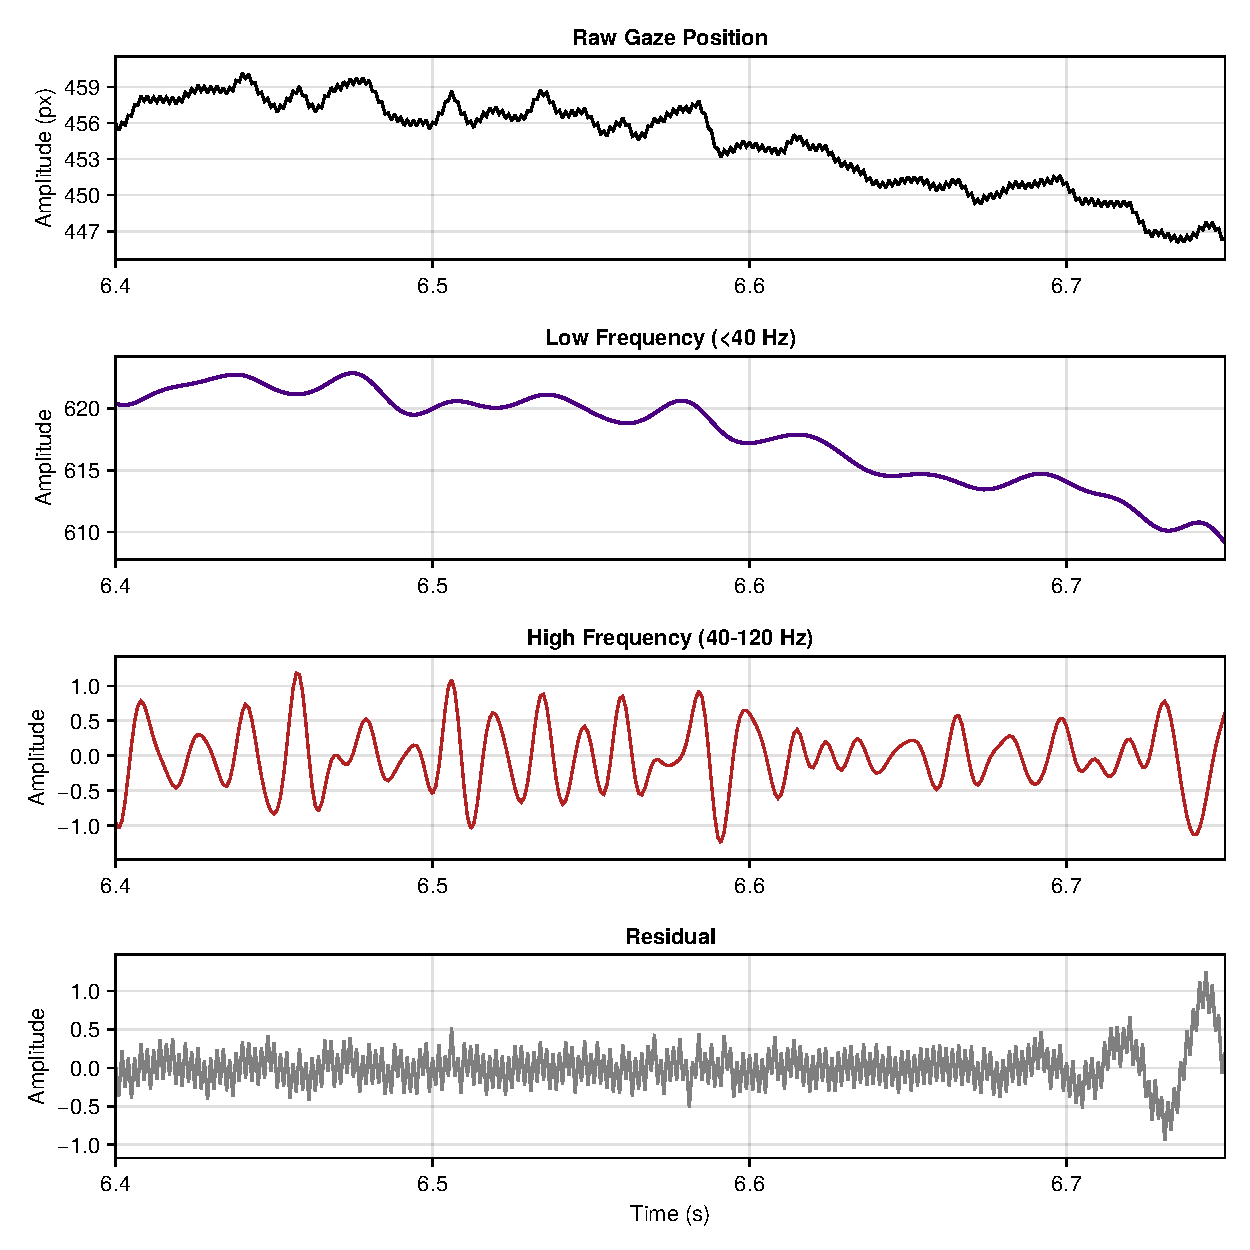
\includegraphics[width=0.95\linewidth]{figures/fixation_decomposition_zoomed.pdf}
    \caption{\textbf{The Fourier decomposition of a typical fixation shows significant OMT contribution.} This typical fixation, with no present microsaccades, provides the context of how high-frequency OMT present in human fixations. There is a clear drift that can be accounted for by band-pass filtering or by examining the velocity. The residuals left by truncating at \qty{120}{\hertz} show no significant biological contribution.}
    \label{fig:fixation_trace}
\end{figure}